\documentclass{ieee}

\usepackage{graphicx}

\title{DARTS and ProxylessNAS Summaries}
\author{Aamir Jamal, Pawan Shetty, Adam Spindler}

\begin{document}
\maketitle

\section{Introduction}
Neural networks are very complicated systems and require a lot of tuning to work properly on certain tasks such as image classification or text classification. Parameters of the networks are learned by using gradient descent to find a minimum of a loss function that describes the error that the network has on a particular set of training data. The architecture of a network, until recently, has been hand crafted by researchers. 

Various techniques have been used to find neural network architectures automatically. Reinforcement learning has been popular for the task, but is extremely computationally expensive requiring on the order of thousands of GPU hours to find a suitable setup. The two papers examined in this work, DARTS \cite{liu2018darts} and ProxylessNAS \cite{cai2018proxylessnas}, propose techniques to create a continuous loss function that includes a representation of the network architecture so that gradient descent can be used to find an optimal architecture in much less time.

\section{ProxylessNAS}
\subsection{Overview}
Although differentiable architecture search is much faster than previous techniques, it requires a lot of GPU memory. Also techniques such as DARTS train their architecture on a smaller, proxy, task like a subset of CIFAR-10. Then they use their same architecture on their true target task such as ImageNet. This means that the architecture was not tailored to the true task that it was meant to solve so it is unlikely to be the best architecture for the job.

ProxylessNAS also learns different architectures for different target hardware. Architectures meant to run on GPUs can take advantage of the parallelism that the hardware provides, but the same architecture would be much slower running on a mobile device. They introduce a differentiable function to model the performance of different devices so that the architecture can be learned for a specific device, GPU, CPU, or mobile. 

\subsection{Architecture Search Setup}
DARTS uses a technique where they train an architecture on a training set, and then evaluate the architecture itself on a validation set. They then differentiate the validation loss with respect to the architecture and make updates accordingly. Each node in the network has a possible set of operations that it could represent, such as a 3x3 convolution or max pooling. They calculate the output of each of these operations and then the architecture representation is used to weight the options to ultimately select the best one. The issue is that the outputs of each of these operations need to be stored in memory. For every N paths through their network representation they must store the feature maps which means they need N times the amount of GPU memory to train their network compared to a regular CNN.

The reason that DARTS is not able to be trained on the true target task is because of the amount of memory that it uses. A full network that would be capable of solving ImageNet cannot be trained for because the feature maps for all of the paths through this large network would have to be stored in memory. They get around this constraint by searching for small components of the network, called blocks, and putting them together to form a larger network. The problem is that this architecture is repeated and not as complex as it could be. The best network for the task most likely is not one that is repeated.

ProxylessNAS uses a similar technique to DARTS for representing the neural network architecture. They have a set of nodes that make up the network and model connections between them as common neural network operations. They construct a network that is much larger than necessary, containing all of the candidate operations connecting each of the nodes together.

The over-parameterized network is much too large to train on using the same technique as DARTS. Instead of using all of the paths in the network at once, they binarize the path weights so that only a single one is used at a time. In their network representation they have weights on all of the paths that connect the nodes together. If the path weight is low, that means the connection is unlikely to be useful. If the path weight is high, then it should be apart of the final architecture. Binarizing the path weights means that they are setting edge weights for the selected path to 1 and all others to 0. Paths are selected randomly throughout the network during training. Using this technique, they save more than an order of magnitude of memory.

As each batch of input data is passed through this model, a new path is randomly selected through the network using the path weights as the distribution to sample from. Then the weight parameters on the currently selected path are updated. So as a batch of image data is passed through the network, the weights of the convolution kernels would be updated. During this part of the training, the architecture parameters remain constant. Then using this path through the network, the loss is calculated on the validation set and the gradient with respect to the architecture parameters is calculated while the weights of the selected path are kept constant. With the gradient computed, the architecture parameters can be updated so now a different path may have higher weights. Freezing one set of weights when training on the other, for example freezing architecture weights when training the network, also helps reduce memory cost.

\subsection{Training for Specific Target Hardware}

To train their architecture for different hardware they attempt to reduce the overall latency of the network, which is the time it takes for a given architecture to predict a result for an input. They choose to use latency instead of FLOPs because GPUs are able to run operations in parallel so FLOPs would not be a good indication of response time on that platform. They model latency as a continuous function of an operation, such as conv 3x3 or max pooling. The latency function can be changed depending on the hardware that is being targeted. The architecture is represented as a set of paths which are made up of these operations. The total latency for the network is the latency of each operation in the over-parameterized network weighted by its probability of ending up in the final architecture. Now the overall latency is a function of the architecture so they can compute the gradient of this function with respect to the architecture to reduce its latency. The latency of the architecture is added to the overall loss function, which gives them the following resulting function. 

\begin{equation}
    L = L_{Cross\_entropy\_validation} + \lambda_1 ||w||_2^2 + \lambda_2Latency()
\end{equation}

In their loss function they include a weight regularization term to ensure that they weights do not become too large, which is a common approach in loss functions for neural networks. The weight regularization and the latency term are multiplied by scale factors which are hyperparameters so the sensitivity of the loss function to the weights and latency can be adjusted.

When searching for architectures on mobile they included various MBConv blocks into the search space which were first introduced in MobileNetV2 \cite{sandler_howard_zhu_zhmoginov_chen_2018}. They are similar to residual blocks in that they have connections between layers that skip a layer in the middle. For MBConv layers though they use layers with fewer filters on the ends and layers with more filters in the middle. The shallower layers on the end with the skip connections do not have a non-linearity applied because more feature information needs to be preserved. On the layers in the middle they use depth-wise separable convolutions which are more efficient than regular convolutions. A depth-wise separable convolution is applied to each each layer depth-wise in the previous layer, where each kernel in the depth direction has different weights. Then a 1x1 convolution is applied across the entire depth of the image. Each 1x1 convolution acts as a different filter, so the number of output channels will be the same as the number of 1x1 convolutions that are used. A depth-wise convolution results in less weights being used overall, so it is faster to compute. \cite{separable_convolutions_2018} MBConv layers used in MobileNetV2 were shown to perform well on mobile devices in terms of speed and accuracy \cite{sandler_howard_zhu_zhmoginov_chen_2018}, which is why they where added to the architecture search space in ProxylessNAS.

\begin{figure}[h]
    \begin{center}
    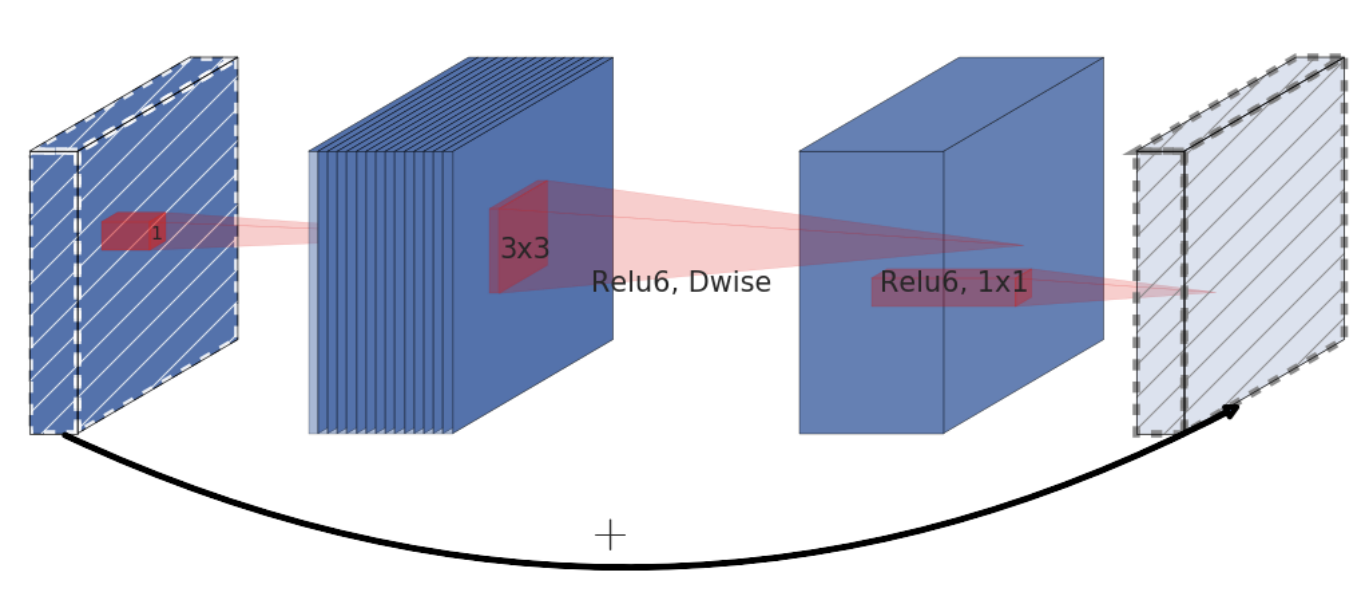
\includegraphics[width=7cm]{images/mbconv.png}
    \end{center}
    \label{mbconv_fig}
    \caption{An MBConv block with a depth-wise convolution applied to the middle layer, split into the 2 steps. The layers with the crosses do not have a non-linearity applied to them. Taken from \cite{sandler_howard_zhu_zhmoginov_chen_2018}}
\end{figure}

\subsection{Results}

The architecture search technique described above was able to achieve state-of-the-art results in a few different categories. On CIFAR-10 it got 2.08\% test error compared to 2.13\% which was achieved by AmoebaNet-B. It is a marginal improvement, but uses only 5.7 million parameters while the other network uses 34.9 million. On ImageNet evaluated on a GPU they also achieve state-of-the-art accuracy, getting 75.1\% while the previous is 72.0\%. When testing ImageNet on a mobile platform they achieve state-of-the-art accuracy when evaluation must be under 80ms getting theirs to run in 78ms and be 74.6\% accurate. Without using their latency regularization, the architecture search finds one with 158ms of latency on the Pixel 1, so it is definitely necessary to explicitly train for it. Their search cost is also much lower than the other methods. It takes 200 GPU hours to search for their architecture while the next best is 40,000 GPU hours. 
\bibliographystyle{unsrt}
\bibliography{sources}
 
\end{document}